\chapter{因果推断}
\label{chap:causal-inference}

第~\ref{chap:mathematical-statistics}章研究怎样从有限观测推断未知总体，第
\ref{chap:information-theory-and-statistical-geometry}章进一步说明观测分布接近会
怎样限制统计区分。即使样本足够多，观测分布也只能告诉我们哪些变量一同出现、在什么
条件下可以相互预测。若问题改成“主动改变一个因素以后，结果会怎样”，推断目标已经
发生变化。接受培训的人平均成绩更高，可能是培训提高了成绩，也可能是基础较好的人更
愿意参加培训；把成绩预测得很准，仍不能区分这两种解释。

本章沿用一个二元处理\(T\)、结果\(Y\)与处理前协变量\(X\)，比较三类问题。
观测问题询问\(p(y\mid t,x)\)，干预问题询问把处理主动设为\(t\)后的结果分布，
反事实问题则询问同一个体在另一处理下会得到什么结果。三者使用相似的条件概率记号，
却依赖不同信息。我们先构造一个无法由观测关联消除的歧义，再分别建立结构因果模型与
潜在结果的表达。随后，调整公式说明哪些假设能够把干预效应化成可观测量；假设不足时，
部分识别保留所有仍与证据相容的答案，而不是用一个点估计掩盖缺失信息。

因果图在本章只承担表达生成假设所需的局部职责。我们会定义有向边、无环生成次序和几种
三节点结构，但不预先使用完整图论。后续图论章将系统建立一般图结构；这里的重点是辨认
每项因果结论究竟由数据、设计还是额外假设支持。

\section{观测关联与生成结构}
\label{sec:causal-observation-generation}

\subsection{观测等价与干预差异}

先忽略协变量，只考虑二元处理\(T\in\{0,1\}\)和二元结果
\(Y\in\{0,1\}\)。设未观测背景变量
\(U\sim\operatorname{Bernoulli}(1/2)\)。下面两套机制都生成
\[
  \mathbb{P}(T=0,Y=0)
  =
  \mathbb{P}(T=1,Y=1)
  =
  \frac12,
\]
而另外两个组合的概率为零。

第一套机制是
\begin{equation}
  T=U,\qquad Y=U.
  \label{eq:causal-observational-equivalence-confounding}
\end{equation}
处理和结果都由共同背景\(U\)决定，改变\(T\)本身不会进入\(Y\)的生成式。第二套机制是
\begin{equation}
  T=U,\qquad Y=T.
  \label{eq:causal-observational-equivalence-effect}
\end{equation}
这里背景决定处理，处理再决定结果。两套机制在自然运行时都只有\(T=Y\)的记录，所以
\[
  \mathbb{P}(Y=1\mid T=1)=1,\qquad
  \mathbb{P}(Y=1\mid T=0)=0.
\]
无论观测样本增加多少，这两个条件概率都完全相同。

现在主动把处理设为\(t\)，同时保留其余生成机制。对式
\eqref{eq:causal-observational-equivalence-confounding}，设置\(T=t\)以后仍有
\(Y=U\)，因而
\[
  \mathbb{P}(Y=1\mid \operatorname{do}(T=t))=\frac12,
  \qquad t\in\{0,1\}.
\]
对式~\eqref{eq:causal-observational-equivalence-effect}，设置处理后有\(Y=t\)，
所以
\[
  \mathbb{P}(Y=1\mid \operatorname{do}(T=t))=t.
\]
两套机制的观测分布相同，干预分布却不同。这是观测与干预的基本反例：关联强度再大，
也不能单独决定改变处理的后果。缺少的不是更精确的分布估计，而是关于变量怎样生成的
约束。

\subsection{结构因果模型与生成机制}

相同观测分布可以来自不同生成机制。要让“替换处理机制”成为明确运算，需要记录变量怎样由直接输入与背景产生，而不只记录联合概率表。
\begin{definition}[无环结构因果模型]
  \label{def:causal-structural-model}
  本章的\term{结构因果模型}（structural causal model, SCM）由内生变量的状态空间、外生背景的联合概率分布以及可测结构函数组成。设内生变量为
\(\bm{V}=(V_1,\ldots,V_d)\)，外生变量为\(\bm{U}\)，模型写成
\begin{equation}
  V_j=f_j(\operatorname{pa}_j,U_j),
  \qquad j=1,\ldots,d,
  \label{eq:causal-scm-definition}
\end{equation}
其中\(\operatorname{pa}_j\)是进入第\(j\)个方程的其他内生变量。外生变量概括模型
未继续解释的背景差异；它们可以相关，此时相关性表示尚未显式展开的共同原因。无环性要求存在节点顺序，使每个函数的内生输入都来自更早的节点。
\end{definition}

若这些方程可以按某个顺序依次求值，且后面的变量不再反过来决定前面的变量，就得到
\term{无环}（acyclic）结构。把每个变量画成节点，并在\(V_k\)进入\(f_j\)时画有向边
\(V_k\to V_j\)，便得到有向无环图。箭头在SCM中表示直接生成输入，而不只是条件分布的
一种分解方式。给定外生变量分布和全部结构方程，按无环次序求值会诱导一个观测联合分布
\scite{math-pearl2009causality}

无环次序还给出解的存在性与唯一性。设节点按
\(V_{j_1},\ldots,V_{j_d}\)排列，使每个父节点都先于其子节点。给定任意外生取值
\(\bm{u}\)，第一个方程只依赖已经给定的外生量，因而唯一确定\(v_{j_1}\)；若前
\(k-1\)个变量已经确定，第\(k\)个方程的全部内生输入也已经确定，于是唯一得到
\(v_{j_k}\)。归纳到\(d\)便得到唯一的\(\bm{v}(\bm{u})\)。外生分布通过映射
\(\bm{u}\mapsto\bm{v}(\bm{u})\)推前，形成观测分布。循环方程没有这种递归保证：
它可能无解或有多个解，必须另外规定平衡选择、动态过程或其他解条件。

\begin{definition}[理想干预]
  \label{def:causal-intervention}
对上述SCM的变量\(T\)作\term{干预}（intervention）
\(\operatorname{do}(T=t)\)，表示删除原来生成\(T\)的结构方程，并用常量方程
\(T=t\)替换；其他方程和外生变量分布保持不变。修改后的模型诱导的结果分布记作\(P^{\operatorname{do}(T=t)}\)。
\end{definition}
对具有密度或质量函数的无环模型，
若各局部机制由相互独立的外生噪声驱动，并且观测分布按因果图分解为
\[
  p(\bm{v})=\prod_{j=1}^{d}p(v_j\mid \operatorname{pa}_j),
\]
则单节点理想干预后的\term{截断分解}为
\begin{equation}
  p(\bm{v}_{-T}\mid\operatorname{do}(T=t))
  =
  \prod_{j:V_j\neq T}
  p(v_j\mid\operatorname{pa}_j)
  \big|_{T=t}.
  \label{eq:causal-truncated-factorization}
\end{equation}
局部因子必须取由结构机制指定的版本。观测联合分布只能在父变量的实际支持上确定这些因子；若干预产生了原来从未出现的父变量组合，任意补出的观测条件分布不能替代结构方程，也不能据此声称效应已由数据识别。

这条公式不是从任意概率图自动得到的。只有当局部条件分布被解释为在干预下保持不变的
生成机制时，删除处理节点的原机制才有因果含义。

固定值干预只是机制替换的一种。\term{随机干预}（stochastic intervention）可以把
处理方程替换为由新外生随机量驱动的规则，使给定处理前信息\(X=x\)时的新分配分布为
\(q(t\mid x)\)。在前述独立外生噪声假设和简单结构\(X\to T\)、\(X\to Y\)、
\(T\to Y\)下，若其余机制保持不变，干预后的联合分布为
\begin{equation}
  p^q(x,t,y)
  =
  p(x)q(t\mid x)p(y\mid t,x).
  \label{eq:causal-stochastic-intervention}
\end{equation}
确定性策略是\(q(\,\cdot\mid x)\)集中在某个动作上的特例。式
\eqref{eq:causal-stochastic-intervention}仍是一项机制假设：策略若同时改变结果测量、
参与人群或其他生成规则，就不能只替换处理因子。

\subsection{共同原因、中介与碰撞点}

三个变量的局部结构已经能说明调整变量时最常见的差别。结构
\[
  T\leftarrow X\to Y
\]
把\(X\)称为\(T\)与\(Y\)的\term{共同原因}（common cause）。即使\(T\)不影响
\(Y\)，不同\(X\)人群采用处理的比例不同，也会使\(T\)与\(Y\)在观测中相关。
这就是混杂产生的一条路径。

结构
\[
  T\to M\to Y
\]
中的\(M\)是\term{中介变量}（mediator）。若目标是处理的总效应，把\(M\)固定后比较
会阻断一部分真实作用；若目标是直接效应，则需要另外定义允许保留或阻断哪些路径。
“加入更多控制变量”因此不是无条件正确的策略。

结构
\[
  T\to C\leftarrow Y
\]
中的\(C\)是\term{碰撞点}（collider），因为两条箭头在它处相遇。未给定\(C\)时，
这条路径不必产生关联；只选择\(C\)取某些值的样本或在回归中给定\(C\)，反而可能使
\(T\)与\(Y\)相关。关联是否出现以及方向如何，取决于具体的选择机制。例如，若两个
独立能力共同决定总分，入选要求总分超过阈值，且两种能力可以相互补偿，那么只考察
已入选者时，一种能力较弱的人往往需要在另一种能力上更强。若入选规则改为两项能力
分别超过各自阈值，这种负关联则未必出现。无论哪种情形，由选择产生的关联都不能
解释为任一能力造成另一能力。

共同原因适合在效应识别时调整，中介是否调整取决于目标，碰撞点通常不应仅因它可观测
就调整。这三种判断依赖箭头的因果语义。若一张有向图只记录
\(p(\bm{v})=\prod_jp(v_j\mid\operatorname{pa}_j)\)，它表达的是概率约束，不能单凭
箭头方向回答式~\eqref{eq:causal-truncated-factorization}中的干预问题。

图~\ref{fig:causal-local-path-patterns}把三种局部结构放在同一视野中。双边框表示把
中间节点加入条件集；共同原因与中介是非碰撞点，给定后会关闭相应路径，碰撞点的行为
恰好相反。
\begin{figure*}[htbp]
  \centering
  \begin{tikzpicture}[figure picture,x=1mm,y=1mm,
    causalnode/.style={circle,draw=FigureStroke,fill=white,line width=1pt,
      minimum size=7mm,inner sep=0pt,font=\figurefont\mdseries\footnotesize},
    conditionednode/.style={causalnode,draw=FigureYellow,
      double=white,double distance=0.7pt},
    causaledge/.style={-{Stealth[length=2.2mm,width=1.4mm]},draw=FigureStroke,line width=1.1pt},
    paneltitle/.style={font=\figurefont\mdseries\footnotesize,text=FigureInk},
    panellabel/.style={font=\figurefont\mdseries\small,text=FigureInk},
    note/.style={font=\figurefont\mdseries\footnotesize,text=FigureMuted,align=center}]

    \draw[FigureMuted,line width=0.6pt] (54,-6)--(54,34);
    \draw[FigureMuted,line width=0.6pt] (108,-6)--(108,34);

    \node[panellabel,anchor=west] at (1,32) {(a)};
    \node[paneltitle] at (27,32) {共同原因};
    \node[conditionednode] (fork-x) at (27,21) {\(X\)};
    \node[causalnode] (fork-t) at (12,10) {\(T\)};
    \node[causalnode] (fork-y) at (42,10) {\(Y\)};
    \draw[causaledge] (fork-x)--(fork-t);
    \draw[causaledge] (fork-x)--(fork-y);
    \node[note] at (27,-2) {给定\(X\)时关闭路径};

    \node[panellabel,anchor=west] at (56,32) {(b)};
    \node[paneltitle] at (81,32) {中介链};
    \node[causalnode] (chain-t) at (64,15) {\(T\)};
    \node[conditionednode] (chain-m) at (81,15) {\(M\)};
    \node[causalnode] (chain-y) at (98,15) {\(Y\)};
    \draw[causaledge] (chain-t)--(chain-m);
    \draw[causaledge] (chain-m)--(chain-y);
    \node[note] at (81,-2) {给定\(M\)时关闭路径};

    \node[panellabel,anchor=west] at (110,32) {(c)};
    \node[paneltitle] at (135,32) {碰撞点};
    \node[causalnode] (collider-t) at (120,21) {\(T\)};
    \node[causalnode] (collider-y) at (150,21) {\(Y\)};
    \node[conditionednode] (collider-c) at (135,10) {\(C\)};
    \draw[causaledge] (collider-t)--(collider-c);
    \draw[causaledge] (collider-y)--(collider-c);
    \node[note] at (135,-2) {不给定时关闭；给定\(C\)时打开};
  \end{tikzpicture}
  \caption{共同原因、中介与碰撞点的局部路径。双边框节点表示已加入条件集，因而图形
  不只依赖颜色传达条件化。面板(a)、(b)中的中间节点是非碰撞点，给定后关闭路径；
  面板(c)中的中间节点是碰撞点，给定后反而打开路径。}
  \label{fig:causal-local-path-patterns}
\end{figure*}

\subsection{d-分离与条件独立}

为了把三节点判断推广到较大的有向图，需要同时检查处理与结果之间的每条路径。设
\(\mathcal{G}=(V,E)\)为有向无环图。这里的\term{路径}（path）是忽略箭头方向后，
由相邻且互不重复的节点组成的序列；只有明确称为\term{有向路径}（directed path）时，
才要求沿箭头方向前进。若从节点\(v\)出发，沿长度至少为一的有向路径能够到达节点
\(w\)，就称\(w\)为\(v\)的\term{后代}（descendant），并称\(v\)为\(w\)的
\term{祖先}（ancestor）。本章的祖先与后代均要求路径长度至少为一，因而不把节点
自身计入其中。

\begin{definition}[活跃路径与d-分离]
  \label{def:causal-d-separation}
  给定条件节点集\(S\subseteq V\)。路径上的内部节点\(v_i\)若在该路径上呈现
  \(v_{i-1}\to v_i\leftarrow v_{i+1}\)，就称为\term{碰撞点}（collider）；否则为
  非碰撞点。路径在给定\(S\)时\term{活跃}（active），当且仅当每个非碰撞点都不在
  \(S\)中，并且每个碰撞点自身或它的至少一个后代在\(S\)中。

  对两两不交的节点集\(A,B,S\subseteq V\)，若连接\(A\)中任一节点与\(B\)中任一
  节点的每条路径都不活跃，就称\(A\)与\(B\)被\(S\)
  \term{d-分离}（d-separated），记为
  \(A\perp_{\mathcal{G}}B\mid S\)；否则称为d-连接。
\end{definition}

这一定义中，给定非碰撞点会关闭路径，给定碰撞点或其后代却会打开原本关闭的路径。
例如，考虑同时含有
\[
  X\to M\to Y,\qquad X\to C\leftarrow Y,\qquad C\to D
\]
的图。\(X\)与\(Y\)之间有经过\(M\)的链式路径和经过\(C\)的碰撞路径。不给定任何
节点时，前一条路径活跃而后一条关闭，所以\(X\)与\(Y\)仍然d-连接。给定
\(S=\{M\}\)会关闭链式路径，碰撞路径也仍关闭，因而
\(X\perp_{\mathcal{G}}Y\mid M\)。若改为给定\(S=\{M,C\}\)，碰撞点\(C\)被打开；
给定\(S=\{M,D\}\)时，\(C\)的后代\(D\)被给定，也会打开同一条路径。这两种情况下
\(X\)与\(Y\)都重新d-连接。这个例子也说明，只检查一条路径是否关闭并不足以判断
d-分离。第~\ref{chap:graph-theory}章将把路径、分离和结构分解放回一般图对象中；
本章只使用有向无环图上的这套条件化判据。

图~\ref{fig:causal-d-separation-paths}画出了条件集\(S=\{M\}\)的情形。经过\(M\)的
链式路径被关闭，经过\(C\)的碰撞路径仍关闭，所以两条路径同时被阻断。
\begin{figure}[htbp]
  \centering
  \begin{tikzpicture}[figure picture,x=1mm,y=1mm,
    causalnode/.style={circle,draw=FigureStroke,fill=white,line width=1pt,
      minimum size=7mm,inner sep=0pt,font=\figurefont\mdseries\footnotesize},
    conditionednode/.style={causalnode,draw=FigureYellow,
      double=white,double distance=0.7pt},
    causaledge/.style={-{Stealth[length=2.2mm,width=1.4mm]},draw=FigureStroke,line width=1.1pt},
    note/.style={font=\figurefont\mdseries\footnotesize,text=FigureMuted,align=center}]

    \node[note,text=FigureInk] at (40,27) {条件集\(S=\{M\}\)};
    \node[causalnode] (dsep-x) at (8,14) {\(X\)};
    \node[conditionednode] (dsep-m) at (40,14) {\(M\)};
    \node[causalnode] (dsep-y) at (72,14) {\(Y\)};
    \node[causalnode] (dsep-c) at (40,-1) {\(C\)};
    \node[causalnode] (dsep-d) at (40,-16) {\(D\)};
    \draw[causaledge] (dsep-x)--(dsep-m);
    \draw[causaledge] (dsep-m)--(dsep-y);
    \draw[causaledge] (dsep-x)--(dsep-c);
    \draw[causaledge] (dsep-y)--(dsep-c);
    \draw[causaledge] (dsep-c)--(dsep-d);
  \end{tikzpicture}
  \caption{多条路径下的d-分离。双边框节点\(M\)属于条件集，因而上方链式路径关闭；
  碰撞点\(C\)及其后代\(D\)均未给定，所以下方路径也关闭。若把\(C\)或\(D\)加入
  条件集，下方路径会重新打开。}
  \label{fig:causal-d-separation-paths}
\end{figure}

\begin{definition}[因果Markov性]
  \label{def:causal-markov-property}
分布\(p\)相对于因果图\(\mathcal{G}\)满足\term{因果Markov性}
（causal Markov property），是指对任意两两不交的节点集\(A,B,S\)，都有
\[
  A\perp_{\mathcal{G}}B\mid S
  \quad\Longrightarrow\quad
  \bm{V}_A\perp\bm{V}_B\mid\bm{V}_S,
\]
其中\(\bm{V}_A\)表示由节点集\(A\)中的随机变量组成的向量，\(\bm{V}_B\)与
\(\bm{V}_S\)同理。
\end{definition}
对有向无环图，这一全局表述等价于局部表述：每个变量在给定其父节点后，与其非后代中
除自身和父节点外的其他变量条件独立。在无环SCM和相互独立的外生噪声条件下，可以沿逆拓扑次序
逐个积分掉无关后代；每次只留下当前节点的条件因子，由此得到局部Markov性和全局
d-分离结论。完整的图分解与消元工具由第~\ref{chap:graph-theory}章继续建立。

\section{干预与潜在结果}
\label{sec:causal-intervention-potential-outcomes}

\subsection{干预分布与条件分布}

观察\(T=t\)会筛选自然机制恰好产生该取值的个体，因此
\[
  p(y\mid T=t)
\]
同时包含处理作用和进入处理组的选择机制。干预
\[
  p(y\mid\operatorname{do}(T=t))
\]
则先切断处理的自然生成机制，再考察其余机制产生的结果。第
~\ref{sec:causal-observation-generation}节的反例具体计算的是事件\(Y=1\)的概率：
两套机制中都有\(\mathbb{P}(Y=1\mid T=t)=t\)；在共同原因机制中，
\(\mathbb{P}(Y=1\mid\operatorname{do}(T=t))=1/2\)，而在直接作用机制中，该概率
等于\(t\)。这些等式说明观察条件分布与干预分布不能通过省略
\(\operatorname{do}\)符号互换。

\subsection{潜在结果与处理效应}

\begin{definition}[潜在结果]
  \label{def:causal-potential-outcomes}
  对已明确的目标总体、处理版本和结果测量时间，\term{潜在结果}（potential outcome）\(Y(t)\)表示把处理设为\(t\)时，该研究单位将
得到的结果。对二元处理，每个单位都有一对数学对象
\[
  (Y(0),Y(1)),
\]
这对对象定义在同一研究单位的背景概率空间上；若借助SCM表示，就在同一个外生背景下分别替换处理方程。
\end{definition}
但实际只能观察当前处理对应的一个结果\scite{math-hernan2020whatif}

\begin{definition}[平均处理效应]
  \label{def:causal-average-treatment-effect}
对二元处理，假设两种干预下的结果都可积，\term{平均处理效应}（average treatment effect, ATE）定义为
\begin{equation}
  \tau
  =
  \mathbb{E}[Y\mid\operatorname{do}(T=1)]
  -
  \mathbb{E}[Y\mid\operatorname{do}(T=0)].
  \label{eq:causal-ate-interventional}
\end{equation}
\end{definition}
它比较两个干预总体的平均结果，并不要求同一时刻让一个个体同时接受两种处理。若目标
总体、处理版本或结果测量时间改变，式~\eqref{eq:causal-ate-interventional}所定义的
量也会改变。

若处理取值属于有限集合\(\mathcal{T}\)，则定义相应的一组潜在结果
\(\{Y(t):t\in\mathcal T\}\)，任意两个处理的平均对比为
\[
  \tau(t,t')
  =
  \mathbb{E}[Y(t)-Y(t')].
\]
多值处理并不只是多写几个二元比较：重叠条件要对目标中使用的每个处理值成立，剂量的
物理含义和允许比较的处理版本也必须一致。连续处理还需要局部支持和相应的平滑条件，
不能直接把每个精确剂量当作拥有正概率的离散组。

个体处理效应是\(Y(1)-Y(0)\)，平均处理效应也可以写成
\begin{equation}
  \tau
  =
  \mathbb{E}[Y(1)-Y(0)]
  =
  \mathbb{E}[Y(1)]-\mathbb{E}[Y(0)].
  \label{eq:causal-ate-potential-outcomes}
\end{equation}
线性期望使第二个等号成立；它没有使无法同时观察的两个个体结果变得可见。

SCM与潜在结果可以在同一机制下对应起来。若结果方程为
\[
  Y=f_Y(T,X,U_Y),
\]
则保持\(X,U_Y\)不变并把处理输入替换为\(t\)，得到
\begin{equation}
  Y(t)=f_Y(t,X,U_Y).
  \label{eq:causal-scm-potential-outcome}
\end{equation}
因此
\[
  \mathcal{L}(Y(t))
  =
  \mathcal{L}(Y\mid\operatorname{do}(T=t)).
\]
潜在结果侧重比较处理方案，SCM还显式说明变量间的生成顺序和连带变化。两种语言能够
描述同一目标，但一个潜在结果表本身未必给出完整的多变量结构方程。

\subsection{一致性、干扰与处理机制}

要把观察结果连接到潜在结果，至少要明确三类条件。
\begin{definition}[处理一致性与无干扰]
  \label{def:causal-consistency-no-interference}
  对明确的处理版本，\term{一致性}（consistency）要求
实际接受处理\(t\)的单位满足
\begin{equation}
  \begin{gathered}
    T=t\Longrightarrow Y=Y(t),\\
    \text{二元处理时，}\quad Y=TY(1)+(1-T)Y(0).
  \end{gathered}
  \label{eq:causal-consistency}
\end{equation}
对\(n\)个单位，无干扰要求每个\(i\)和任意两个处理向量\(\bm t,\bm t'\)只要\(t_i=t_i'\)，就有\(Y_i(\bm t)=Y_i(\bm t')\)。因此单位\(i\)的潜在结果才可简记为\(Y_i(t_i)\)。这些相等关系按几乎必然意义理解。
\end{definition}
一致性说明观测结果等于实际处理对应的潜在结果。若“接受培训”包含时长、教师和课程完全
不同的版本，却仍用一个二元\(T\)表示，一致性可能没有良好定义。

无干扰要求一个单位的结果不随其他单位的处理改变。若有\(n\)个单位，更一般的潜在结果
应写成\(Y_i(\bm{t})\)，而不是只写\(Y_i(t_i)\)。疫苗、社交网络和市场竞争中，
一个人的处理会改变他人的暴露或机会，无干扰通常不成立。此时需要定义分组、网络暴露
或总体处理比例，不能继续把单个处理变量的ATE解释为全部作用。

“稳定单位处理值”常把处理版本唯一性与无干扰合在一起。它们与处理分配机制仍是不同
条件。分配机制规定\(T\)怎样依赖\(X,Y(0),Y(1)\)等变量；一致性只连接已经接受的处理
与观察结果，并不保证处理像随机试验那样分配。即使处理定义清楚且单位互不干扰，主动
选择处理的人仍可能与未选择者具有不同潜在结果。

\section{因果效应的识别条件}
\label{sec:causal-effect-identification}

前两节已经定义干预目标，却没有保证观测数据能确定它。
本节把生成模型限制、处理分配和支持条件逐项加入，说明何时不同的相容机制必须给出同一目标。
一旦获得识别式，有限样本估计才回到数理统计中的误差问题；增加样本不能替代这一步。

\subsection{识别、估计与计算}

定义~\ref{def:statistics-identifiability}把目标可识别性表述为“同一观测分布对应同一目标值”。这里模型索引是完整生成机制，观测分布只记录自然处理下可看到的量；给定一组模型假设，若所有产生同一可观测分布的允许机制都给出相同因果目标值，就称该目标\term{可识别}（identifiable）。识别是总体层面的唯一确定性。它不表示有限样本估计
已经准确，也不表示求解某个估计式的优化算法一定稳定。反过来，一个算法可以精确拟合
全部观测条件分布，却因第~\ref{sec:causal-observation-generation}节的两套机制而无法
确定干预效应。

随机试验通过设计建立识别。若处理由独立随机装置分配，且两种处理都有正概率，则
\[
  (Y(0),Y(1))\perp T.
\]
结合一致性，对\(t\in\{0,1\}\)和任意可测集合\(B\)有
\begin{equation}
  \mathbb{P}(Y(t)\in B)
  =
  \mathbb{P}(Y(t)\in B\mid T=t)
  =
  \mathbb{P}(Y\in B\mid T=t).
  \label{eq:causal-randomization-marginal-distribution}
\end{equation}
第一步使用随机分配，第二步使用一致性。因此，随机试验识别每个潜在结果的完整边缘
分布；它并不据此识别\(Y(0)\)与\(Y(1)\)在同一个体上的联合分布。结果可积时，取
均值得到
\[
\begin{aligned}
  \mathbb{E}[Y(t)]
  &=
  \mathbb{E}[Y(t)\mid T=t]\\
  &=
  \mathbb{E}[Y\mid T=t].
\end{aligned}
\]
处理组与对照组的均值差因而识别ATE。若存在失访、不依从、处理溢出或随机化后选择
样本，原有独立性需要按实际分析目标重新检查。

\subsection{条件交换性与支持重叠}

观察研究常希望用处理前协变量\(X\)解释分配差异。变量\(X\)必须在所比较的处理下保持相同，不能把处理影响后的结果当成共同分层依据。
\begin{definition}[条件交换性]
  \label{def:causal-conditional-exchangeability}
对二元处理，\term{条件交换性}（conditional exchangeability）要求
\begin{equation}
  (Y(0),Y(1))\perp T\mid X.
  \label{eq:causal-conditional-exchangeability}
\end{equation}
\end{definition}
它表示在固定\(X\)以后，处理组和未处理组的潜在结果分布可以交换。白话地说，\(X\)
已经包含同时影响处理选择和结果的共同原因。该条件涉及无法同时观察的潜在结果，不能
仅凭处理预测准确率或结果拟合误差从数据中验证。

\begin{definition}[二元处理的支持重叠]
  \label{def:causal-overlap}
对需要同时比较两种处理的目标总体，\term{支持重叠}（overlap），也称\term{正值性}（positivity），定义如下。记倾向概率
\[
  e(x)=\mathbb{P}(T=1\mid X=x).
\]
对目标总体中几乎处处的\(x\)，要求
\begin{equation}
  0<e(x)<1.
  \label{eq:causal-overlap}
\end{equation}
\end{definition}
若某类人必然接受或必然不接受处理，观测数据便没有该类人在另一处理下的参照。交换性
说明现有参照为何可比，重叠说明参照确实存在；两者不能互相替代。

正值性的作用域由目标决定，不是要求数据在所有可能协变量和行动上处处有正密度。识别
\(\mathbb{E}[Y(1)]\)只要求目标总体几乎处处满足\(e(x)>0\)，识别
\(\mathbb{E}[Y(0)]\)只要求\(e(x)<1\)，而目标总体ATE同时需要两侧条件。对随机目标
策略\(q(t\mid x)\)，相应要求是：只要目标策略在目标总体的某个\(x\)上给行动\(t\)
正概率，观测分配机制也必须给该行动正概率。目标总体支持之外的\(x\)或目标策略从不采用
的行动不在这项要求内。接近零但不等于零的倾向概率不会破坏总体层面的点识别，却会产生
大权重和有限样本不稳定；这属于可估计性与精度问题。

\subsection{调整公式的推导}

在一致性、条件交换性和重叠成立时，对\(t\in\{0,1\}\)，全期望公式给出
\[
  \mathbb{E}[Y(t)]
  =
  \mathbb{E}_X\bigl[
    \mathbb{E}[Y(t)\mid X]
  \bigr].
\]
条件交换性允许在内层加入实际处理条件：
\[
  \mathbb{E}[Y(t)\mid X]
  =
  \mathbb{E}[Y(t)\mid T=t,X].
\]
重叠保证右侧在目标总体所需的\(X\)取值上由相应处理组定义，一致性再把潜在结果换成
观察结果。于是
\begin{equation}
  \mathbb{E}[Y(t)]
  =
  \mathbb{E}_X\bigl[
    \mathbb{E}[Y\mid T=t,X]
  \bigr].
  \label{eq:causal-g-formula}
\end{equation}
这就是单时点处理的调整公式。令
\(\mu_t(x)=\mathbb{E}[Y\mid T=t,X=x]\)，ATE被识别为
\begin{equation}
  \tau
  =
  \mathbb{E}_X[\mu_1(X)-\mu_0(X)].
  \label{eq:causal-ate-adjustment}
\end{equation}

同一目标还可写成逆概率加权形式。利用条件期望，对处理组有
\[
\begin{aligned}
  \mathbb{E}\left[\frac{TY}{e(X)}\middle|X\right]
  &=
  \frac{\mathbb{P}(T=1\mid X)}{e(X)}
  \mathbb{E}[Y\mid T=1,X]\\
  &=\mu_1(X).
\end{aligned}
\]
对未处理组同理可得
\[
  \mathbb{E}\left[
    \frac{(1-T)Y}{1-e(X)}
    \middle|X
  \right]
  =\mu_0(X).
\]
再取总体期望，得到
\begin{equation}
  \tau
  =
  \mathbb{E}\left[
    \frac{TY}{e(X)}
    -
    \frac{(1-T)Y}{1-e(X)}
  \right].
  \label{eq:causal-ipw-identification}
\end{equation}
调整公式与加权公式是同一识别关系的两种表示。有限样本中如何估计\(\mu_t\)或\(e\)、
怎样交叉拟合以及如何报告不确定性，属于估计问题；它们不能修复交换性错误或支持缺口。

\subsection{后门准则与调整变量}

潜在结果条件交换性直接说明调整公式为何成立，但它没有告诉我们应把哪些变量放进
\(X\)。在具有生成语义的DAG中，从\(T\)到\(Y\)且第一条边指向\(T\)的路径称为
\term{后门路径}（back-door path）；它描述处理自然生成机制与结果之间的非因果联系。
\begin{definition}[单处理、单结果的后门准则]
  \label{def:causal-backdoor-criterion}
  设\(T,Y\)是因果DAG中的不同节点，\(Z\)是与\(\{T,Y\}\)不交的节点集合。若\(Z\)不含\(T\)的后代，且给定\(Z\)阻断\(T\)与\(Y\)之间所有第一条边指向\(T\)的路径，则称\(Z\)满足相对于\((T,Y)\)的\term{后门准则}（back-door criterion）。
\end{definition}
这里的“阻断”
按定义~\ref{def:causal-d-separation}判断，因而把碰撞点放入\(Z\)可能打开路径。

最基本的代表图为\(Z\to T\)、\(Z\to Y\)、\(T\to Y\)。其观测分解是
\[
  p(z,t,y)=p(z)p(t\mid z)p(y\mid t,z).
\]
执行\(\operatorname{do}(T=t)\)时删除\(p(t\mid z)\)，再对\(Z\)积分，得到
\begin{equation}
  p(y\mid\operatorname{do}(T=t))
  =
  \int p(y\mid t,z)p(z)\,\mathrm{d}z.
  \label{eq:causal-backdoor-adjustment}
\end{equation}
一般后门准则把同一推导推广到多条路径：\(Z\)阻断所有进入\(T\)的非因果路径，使给定
\(Z\)后的处理比较不再携带这些路径造成的差异；\(Z\)又不是处理后代，所以干预不会
先改变用于平均的\(p(z)\)。在因果Markov性和所声明DAG包含相关共同原因等条件下，
这给出式~\eqref{eq:causal-backdoor-adjustment}。

三个局部图可以核对这项准则。在\(T\leftarrow X\to Y\)中，\(X\)阻断后门路径；
在\(T\to M\to Y\)中，\(M\)是处理后代，调整它会改变总效应目标；在
\(T\to C\leftarrow Y\)中，空集已经关闭碰撞路径，加入\(C\)反而将其打开。
因此，“处理前测量”“与结果相关”或“能提高预测精度”都不是充分的调整标准。后门
准则是充分条件而不是识别的必要条件；它失败时，随机设计、其他图识别规则或更具体的
结构假设仍可能识别目标。

\subsection{混杂偏差与调整算例}

设\(X\in\{0,1\}\)表示处理前风险，且
\(\mathbb{P}(X=1)=1/2\)。高风险者更常接受处理：
\[
  e(1)=0.8,\qquad e(0)=0.2.
\]
假定给定\(X\)后处理满足交换性，并设潜在结果均值为
\[
\begin{array}{c|cc}
  &X=0&X=1\\ \hline
  \mathbb{E}[Y(0)\mid X]&0.1&0.5\\
  \mathbb{E}[Y(1)\mid X]&0.3&0.7
\end{array}
\]
这些数值是教学构造，不代表真实试验。两个风险层中的处理效应都为\(0.2\)，因此
\[
  \tau
  =
  \frac12(0.3-0.1)+\frac12(0.7-0.5)
  =0.2.
\]

若直接比较观测组均值，Bayes公式给出
\[
  \mathbb{P}(X=1\mid T=1)=0.8,\qquad
  \mathbb{P}(X=1\mid T=0)=0.2.
\]
结合一致性与交换性，
\[
\begin{aligned}
  \mathbb{E}[Y\mid T=1]
  &=0.8\times0.7+0.2\times0.3=0.62,\\
  \mathbb{E}[Y\mid T=0]
  &=0.2\times0.5+0.8\times0.1=0.18.
\end{aligned}
\]
观测均值差为\(0.44\)，明显大于真实ATE \(0.2\)。差异来自处理组包含更多高风险者，
而不是处理效应在计算中突然增大。

按式~\eqref{eq:causal-ate-adjustment}在每个风险层内先比较，再按目标总体的
\(X\)分布平均，便恢复\(0.2\)。这个算例同时显示三项条件的职责：一致性把各组观察
结果连接到相应潜在结果，交换性使同一风险层中的两组可比，重叠保证每层都有两种处理。
若遗漏了未记录的病情严重程度，交换性可能失败；若\(e(1)=1\)，高风险层的未处理结果
便没有观测参照。更灵活的预测模型只能降低已识别表达式的拟合误差，不能消除这两类问题。

\section{部分识别与敏感性分析}
\label{sec:causal-partial-identification-sensitivity}

\subsection{识别集合与观测兼容性}

点识别要求所有允许机制给出同一个目标值。若观测分布和当前假设只把目标限制在一个集合
内，就得到\term{部分识别}（partial identification）。
\begin{definition}[识别集合]
  \label{def:causal-identified-set}
设
\(\mathcal{M}(P_{\mathrm{obs}})\)为与观测分布及已声明假设相容的机制集合，目标泛函为
\(\tau(M)\)。其\term{识别集合}（identified set）定义为
\begin{equation}
  \mathcal{I}(P_{\mathrm{obs}})
  =
  \{\tau(M):M\in\mathcal{M}(P_{\mathrm{obs}})\}.
  \label{eq:causal-identified-set}
\end{equation}
\end{definition}
若相容机制集合为空，说明观测分布与已声明假设不相容；下文讨论其非空情形。一般识别集合不必是单个区间，也可能由彼此分离的点或区间组成。它的下确界与上确界
只确定最小的区间包络，不能证明包络中的每个值都由相容机制达到。下文只有在能够说明
中间值可达时，才把上下界之间的整个区间视为识别集合；否则只报告上下界。区间包络的
宽度可以概括信息与假设留下的总体歧义，但不能替代集合本身。增加样本可以更精确地
估计\(P_{\mathrm{obs}}\)，却不一定使\(\mathcal{I}\)缩成一点。

\subsection{有界结果下的效应界}

先假设二元处理，并且对每个\(t\in\{0,1\}\)都有
\(0\leq Y(t)\leq1\)几乎处处成立；一致性使观测结果也继承这一范围。以下只采用
一致性，不假设交换性。处理下的平均潜在结果可分解为
\[
\begin{aligned}
  \mathbb{E}[Y(1)]
  &=
  \mathbb{E}[TY(1)]
  +
  \mathbb{E}[(1-T)Y(1)]\\
  &=
  \mathbb{E}[TY]
  +
  \mathbb{E}[(1-T)Y(1)].
\end{aligned}
\]
第二项对应未处理者若接受处理会怎样，数据没有观察到它。由
\(0\leq Y(1)\leq1\)，
\[
  0
  \leq
  \mathbb{E}[(1-T)Y(1)]
  \leq
  \mathbb{P}(T=0),
\]
所以
\begin{equation}
  \mathbb{E}[TY]
  \leq
  \mathbb{E}[Y(1)]
  \leq
  \mathbb{E}[TY]+\mathbb{P}(T=0).
  \label{eq:causal-bounded-outcome-y1}
\end{equation}
同理，
\begin{equation}
  \mathbb{E}[(1-T)Y]
  \leq
  \mathbb{E}[Y(0)]
  \leq
  \mathbb{E}[(1-T)Y]+\mathbb{P}(T=1).
  \label{eq:causal-bounded-outcome-y0}
\end{equation}
用第一个区间下端减第二个区间上端得到ATE下界，反向组合得到上界：
\begin{align}
  \mathbb{E}[TY]
  -\mathbb{E}[(1-T)Y]
  -\mathbb{P}(T=1)
  \leq \tau
  \leq{}&
  \mathbb{E}[TY]
  +\mathbb{P}(T=0)\notag\\
  &-\mathbb{E}[(1-T)Y].
  \label{eq:causal-manski-ate-bounds}
\end{align}
这组界可能很宽，但每个端点都有明确依据，而且在当前不受其他限制的机制类中是下面意义下的锐界。
\begin{definition}[相容机制类中的锐界]
  \label{def:causal-sharp-bounds}
对非空相容机制类\(\mathcal M(P_{\mathrm{obs}})\)与实值目标\(\tau(M)\)，若下界与上界分别等于\(\inf_{M\in\mathcal M}\tau(M)\)和\(\sup_{M\in\mathcal M}\tau(M)\)，就称它们是该机制类中的\term{锐界}（sharp bounds）。端点可以由机制达到，也可以仅由相容机制序列任意逼近。
\end{definition}
锐界表示在当前信息下不能再收紧端点，不自动表示两个端点之间的每个值都可实现。本例还能直接构造达到端点的机制：要达到ATE下界，可令所有未处理者的缺失结果
\(Y(1)=0\)，并令所有已处理者的缺失结果\(Y(0)=1\)；要达到上界，则分别令这两类
缺失结果为\(1\)和\(0\)。这些赋值不改变任何已观察结果，并分别达到式
\eqref{eq:causal-manski-ate-bounds}的两个端点。对端点构造作随机混合还能得到中间值，
所以该宽度不是推导松弛造成的。若再要求单调性、函数平滑或特定联合结构，这些端点可能
不再可达，锐界必须相对于缩小后的模型类重新计算。用处理组均值差替代这组界，相当于
偷偷加入交换性，而不是让结论更精确。

\subsection{支持缺口与总体效应界}

现在假设条件交换性在概念上可信，但重叠只在协变量区域
\(\mathcal{O}\)成立。令\(\mathcal{U}\)为目标总体中缺少某种处理的区域，并设
\(\mathcal{O}\mathbin{\dot\cup}\mathcal{U}\)覆盖目标总体。继续假设对所有
\(t\in\{0,1\}\)都有\(0\leq Y(t)\leq1\)几乎处处成立，则条件效应
\[
  \tau(x)=\mathbb{E}[Y(1)-Y(0)\mid X=x]
\]
总在\([-1,1]\)内。在\(\mathcal{O}\)上用调整公式识别它，在
\(\mathcal{U}\)上只保留范围，于是
\begin{align}
  &\mathbb{E}\bigl[
    \tau(X)\mathbb{I}\{X\in\mathcal{O}\}
  \bigr]
  -\mathbb{P}(X\in\mathcal{U})
  \leq \tau \notag\\
  &\qquad\leq
  \mathbb{E}\bigl[
    \tau(X)\mathbb{I}\{X\in\mathcal{O}\}
  \bigr]
  +\mathbb{P}(X\in\mathcal{U}).
  \label{eq:causal-overlap-gap-bounds}
\end{align}
缺口人群占比越大，最坏范围越宽。若愿意把目标总体限制到\(\mathcal{O}\)，可以点识别
重叠人群效应，但它已不是原总体ATE。若假设缺口区域的效应与邻近区域平滑、同号或有
已知范围，界可以收紧；这些都是新增外推假设，不能由重叠区域的拟合优度证明。

\subsection{覆盖缺口与策略价值界}

同一分解可以直接用于单步策略评价。令有限动作集合为\(\mathcal{A}\)，日志策略的动作
概率为\(e_a(x)=\mathbb{P}(T=a\mid X=x)\)，目标策略为\(\pi(a\mid x)\)。假设对
所有\(a\in\mathcal{A}\)都有\(L\leq Y(a)\leq H\)几乎处处成立；一致性使观测结果
也满足同一范围。目标策略价值定义为按\(\pi\)重新分配动作后的平均结果
\[
  V(\pi)
  =
  \mathbb{E}_X\left[
    \sum_{a\in\mathcal{A}}\pi(a\mid X)\mathbb{E}[Y(a)\mid X]
  \right].
\]
在一致性、给定\(X\)的交换性以及
\(\pi(a\mid x)>0\Longrightarrow e_a(x)>0\)成立时，
\[
\begin{aligned}
  \mathbb{E}\left[
    \frac{\pi(T\mid X)}{e_T(X)}Y
    \middle|X
  \right]
  &=
  \sum_{\substack{a\in\mathcal{A}\\ e_a(X)>0}}
  e_a(X)\frac{\pi(a\mid X)}{e_a(X)}
  \mathbb{E}[Y\mid T=a,X]\\
  &=
  \sum_{a\in\mathcal{A}}
  \pi(a\mid X)\mathbb{E}[Y(a)\mid X].
\end{aligned}
\]
对\(X\)再取期望，便得到
\begin{equation}
  V(\pi)
  =
  \mathbb{E}\left[
    \frac{\pi(T\mid X)}{e_T(X)}Y
  \right].
  \label{eq:causal-policy-value-weighting}
\end{equation}
这正是换测度在因果目标上的使用：权重改变动作分配，却保留给定背景和动作的结果机制。
等式中的随机权重只在日志实际可能选择的动作上求值；目标策略在其余动作上的概率由覆盖
条件强制为零，因而没有\(0/0\)的约定。

若覆盖条件失败，定义目标策略落在缺口上的概率质量
\[
  r
  =
  \mathbb{E}_X\left[
    \sum_{a:e_a(X)=0}\pi(a\mid X)
  \right],
\]
并记已覆盖部分能够识别的贡献为
\[
  K
  =
  \mathbb{E}_X\left[
    \sum_{a:e_a(X)>0}
    \pi(a\mid X)\mathbb{E}[Y\mid T=a,X]
  \right].
\]
缺口部分只能贡献\([Lr,Hr]\)，从而
\begin{equation}
  K+Lr
  \leq
  V(\pi)
  \leq
  K+Hr.
  \label{eq:causal-policy-value-bounds}
\end{equation}
两个策略各自的价值上下界若分离，现有信息仍足以确定其排序；若相应范围重叠，单独比较
这两组边际上下界不足以判断排序。此时应直接研究
\(V(\pi_1)-V(\pi_2)\)的联合识别集合或上下界，因为两个策略共享同一组未知潜在结果，
不能把它们的边际范围当作彼此独立。无论如何，都不能把某个拟合器的单一外推当作
排序证据。这里讨论的是单步行动。
第~\ref{sec:decision-dynamic-programming}节建立序贯策略与状态价值后，还要逐时刻检查历史
覆盖、时间变化的混杂和轨迹结果定义，不能把式~\eqref{eq:causal-policy-value-weighting}
直接套到整条轨迹。

图~\ref{fig:causal-confounding-coverage}把两种识别障碍分别数值化。左图是前面的混杂例子；右图另构一个单步策略族：结果位于\([0,1]\)，已覆盖部分的条件平均收益始终为\(0.6\)，未覆盖目标质量为\(r\)，于是\(K=0.6(1-r)\)。当\(r=0.2\)时，价值只能限制在\([0.48,0.68]\)。这段宽度\(0.2\)来自缺口中的结果机制未被观测，并不是通过增加同一覆盖区域内的样本就能消除的置信误差。

\begin{figure*}[htbp]
  \centering
  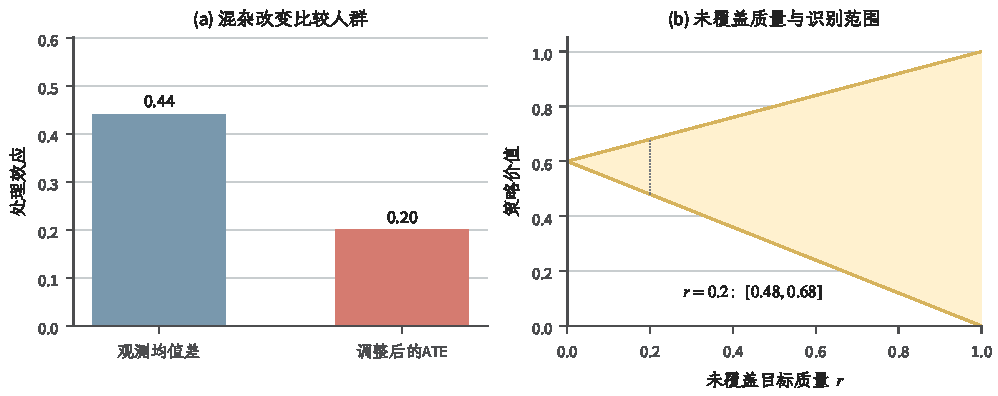
\includegraphics[width=\linewidth]{figures/math-preparation/probability-discrete/causal-confounding-coverage.pdf}
  \caption{两个独立的因果教学构造。左图复用混杂算例，比较观测均值差\(0.44\)与调整后的ATE \(0.20\)。右图假定结果范围为\([0,1]\)、已覆盖部分平均收益为\(0.6\)，绘制式~\eqref{eq:causal-policy-value-bounds}的范围\([0.6(1-r),0.6(1-r)+r]\)。阴影是总体识别范围，不是抽样置信带；两面板也不表示同一数据集。}
  \label{fig:causal-confounding-coverage}
\end{figure*}

\subsection{线性混杂与潜在结果偏差函数}

未观测混杂留下的歧义可以用敏感性参数表达，而不必在“完全无混杂”和“完全不可知”
之间二选一。一个最小线性例子先显示偏差从哪里进入。设变量已经中心化，并令
\[
  T=\alpha U+\varepsilon_T,\qquad
  Y=\beta T+\gamma U+\varepsilon_Y,
\]
其中\(U,\varepsilon_T,\varepsilon_Y\)两两独立、方差有限，且
\(\operatorname{Var}(T)>0\)。把\(Y\)仅对\(T\)作总体线性回归，观测斜率为
\begin{equation}
  \beta_{\mathrm{obs}}
  =
  \frac{\operatorname{Cov}(T,Y)}{\operatorname{Var}(T)}
  =
  \beta+
  \gamma\frac{\alpha\operatorname{Var}(U)}{\operatorname{Var}(T)}.
  \label{eq:causal-linear-confounding-bias}
\end{equation}
\(\beta\)是该结构模型中的处理系数，后一项是共同原因同时进入处理和结果造成的混杂
偏差。若领域信息只支持该偏差的绝对值不超过\(\Lambda\)，则
\(\beta\in[\beta_{\mathrm{obs}}-\Lambda,\beta_{\mathrm{obs}}+\Lambda]\)。数据可估计
\(\beta_{\mathrm{obs}}\)，却不能在没有额外信息时把\(\alpha,\gamma\)各自分开；改变
函数形式也会改变这个敏感性参数的含义。

对非线性和异质效应，不存在一个普遍通用的斜率修正量。仍记
\[
  \mu_t(x)=\mathbb{E}[Y\mid T=t,X=x],\qquad
  e(x)=\mathbb{P}(T=1\mid X=x).
\]
对目标总体中满足\(0<e(x)<1\)且下列条件期望有限的\(x\)，定义两个选择偏差函数
\begin{align*}
  b_1(x)
  &=
  \mathbb{E}[Y(1)\mid T=1,X=x]
  -
  \mathbb{E}[Y(1)\mid T=0,X=x],\\
  b_0(x)
  &=
  \mathbb{E}[Y(0)\mid T=1,X=x]
  -
  \mathbb{E}[Y(0)\mid T=0,X=x].
\end{align*}
完整条件交换性~\eqref{eq:causal-conditional-exchangeability}蕴含
\(b_1(x)=b_0(x)=0\)。对本节的平均效应目标，后一个条件表达的是较弱的条件均值
交换性；它不能反推出两个处理组中的潜在结果完整条件分布相同。若要对目标总体平均，
上述重叠和有限期望条件还须对目标总体中的\(x\)几乎处处成立。一致性给出
\(\mathbb{E}[Y(1)\mid T=1,X=x]=\mu_1(x)\)，因而
\[
\begin{aligned}
  \mathbb{E}[Y(1)\mid X=x]
  &=
  e(x)\mu_1(x)
  +(1-e(x))\bigl(\mu_1(x)-b_1(x)\bigr)\\
  &=
  \mu_1(x)-(1-e(x))b_1(x).
\end{aligned}
\]
同理，
\[
  \mathbb{E}[Y(0)\mid X=x]
  =
  \mu_0(x)+e(x)b_0(x).
\]
所以条件效应满足
\begin{equation}
  \tau(x)
  =
  \mu_1(x)-\mu_0(x)
  -(1-e(x))b_1(x)-e(x)b_0(x).
  \label{eq:causal-selection-bias-function}
\end{equation}

若领域知识只支持
\[
  |b_1(x)|\leq\Gamma_1(x),\qquad
  |b_0(x)|\leq\Gamma_0(x),
\]
则由三角不等式，
\begin{align}
  \mu_1(x)-\mu_0(x)-\Delta(x)
  \leq\tau(x)
  \leq
  \mu_1(x)-\mu_0(x)+\Delta(x),
  \label{eq:causal-sensitivity-bounds}
\end{align}
其中
\[
  \Delta(x)
  =
  (1-e(x))\Gamma_1(x)+e(x)\Gamma_0(x).
\]
对\(X\)取平均便得到ATE的敏感性区间。这里的\(\Gamma_t\)不是由观测数据自动估计出的
误差条，而是对未观测选择差异强度的假设。敏感性分析应展示结论在多大
\(\Gamma_t\)下改变符号或越过决策阈值，而不是只报告一个方便的参数值。

\subsection{额外假设与识别集合收缩}

若有理由相信处理对每个单位都不会降低结果，即
\[
  Y(1)\geq Y(0),
\]
则ATE至少为零，可以把任何已有下界提高到零。这项\term{单调性}（monotonicity）
排除了受处理伤害的机制；它比“平均上看有益”更强。若只知道处理效应位于
\([-\rho,\rho]\)，则支持缺口中的\([-1,1]\)可替换为更窄范围。

跨环境信息也可能收紧识别集合。例如一个环境提供随机试验，另一个环境只提供目标总体
协变量分布；若条件处理效应在两环境间保持不变，并且协变量支持得到覆盖，就能把试验
效应重新加权到目标环境。机制不变、总体可比和支持覆盖分别是新增假设。仅观察到某个
预测关系在多个环境都稳定，不足以排除共同隐藏原因、选择机制或多个机制恰好同时变化。

识别集合及其区间包络还必须与\term{置信区间}区分。前者在总体分布已知时仍可能不是
单点，表达机制歧义；后者由有限样本产生，表达对总体量、识别集合或其端点的估计误差。
实际报告可以给出端点的置信范围，但不能把包络宽度与抽样误差合并后统一称为“模型
不确定性”，否则读者无法判断增加样本、改变设计或增加假设中的哪一种能够收紧结论。

\section{反事实与行动补救}
\label{sec:causal-counterfactual-recourse}

部分识别讨论总体效应还可能有哪些值。下面改变目标为一个已观测个体的另一种结果，
需要在实际世界和替代行动之间保持同一个外生背景。总体干预边缘不能确定这种配对，
因此即使总体效应已识别，个体反事实仍可能需要更强机制假设。

\subsection{反事实推断与个体背景}

总体干预分布重新从外生背景总体中抽取个体，回答“若所有人采用处理\(t\)，平均会怎样”。
\begin{definition}[SCM中的反事实变量]
  \label{def:causal-counterfactual}
  设无环SCM的自然解映射为\(F\)，行动\(a\)替换指定结构方程后得到解映射\(F^a\)。在同一个外生背景\(\bm U\)上，\term{反事实}（counterfactual）变量定义为\(\bm V_a=F^a(\bm U)\)。给定实际证据\(\bm E\)后的反事实分布，是\(\bm V_a\)关于该证据的条件分布，而不是重新从背景总体抽取\(\bm U\)。
\end{definition}
它以已经观察到的个体为条件，回答“这个人在另一种处理下会怎样”。在SCM中，标准计算包含三个步骤：
\begin{enumerate}
  \item 根据实际观测更新外生背景\(\bm{U}\)的条件分布；
  \item 用目标行动替换相应结构方程；
  \item 在同一个背景分布下运行修改后的方程并计算结果。
\end{enumerate}
这三个步骤常称为背景推断、行动和预测。关键是实际世界与反事实世界共享同一外生背景；
若重新抽取一个人，计算的便是干预总体而不是个体反事实。

这三步可以统一写成分布推前。设无环SCM在自然机制下的解映射为
\(\bm{V}=F(\bm{U})\)，事实证据为\(\bm{E}=\bm{e}\)，行动\(a\)替换若干结构方程后得到
解映射\(F^a\)。若所在空间允许选取正则条件分布
\(P_{\bm{U}\mid\bm{E}=\bm{e}}\)，则对任意可测集合\(B\)，
\begin{equation}
  \begin{aligned}
  \mathbb{P}(\bm{V}_a\in B\mid\bm{E}=\bm{e})
  &=
  \left(F^a_{\#}
    P_{\bm{U}\mid\bm{E}=\bm{e}}\right)(B)\\
  &=
  \int
  \mathbb{I}\{F^a(\bm{u})\in B\}\,
  P_{\bm{U}\mid\bm{E}=\bm{e}}(\mathrm d\bm{u}).
  \end{aligned}
  \label{eq:causal-counterfactual-pushforward}
\end{equation}
其中\(F^a_{\#}P\)表示把分布\(P\)经映射\(F^a\)推前。第一步由事实证据更新背景分布，
第二步只改变映射，第三步把同一个背景后验推到反事实结果空间。连续证据点通常概率为零，
此时等式按正则条件分布的版本理解，并只保证对证据分布几乎处处的\(\bm{e}\)成立。零概率证据点的具体条件值还需要指定版本或额外结构，不能由条件概率的积分恒等式唯一决定。

考虑教学模型
\begin{equation}
  X=U_X,\qquad
  T=f_T(X,U_T),\qquad
  Y=2X+3T+U_Y.
  \label{eq:causal-counterfactual-linear-example}
\end{equation}
某人实际观测为\(X=2,T=0,Y=5\)。由结果方程反推出
\(U_Y=5-2\times2-3\times0=1\)。若保持该人的\(X,U_Y\)不变，把处理设为\(1\)，
则
\[
  Y_{T\leftarrow1}=2\times2+3\times1+1=8.
\]
差值\(3\)来自该结构方程中处理的直接作用。若结果方程或\(U_Y\)不能由观测唯一确定，
反事实结果应是条件分布或取值范围，而不是强行给出\(8\)这样的点值。

\begin{example}[两点背景后验的反事实推前]
  \label{ex:causal-two-point-background-posterior}
  令背景变量\(U\in\{u_{\mathrm L},u_{\mathrm H}\}\)的先验概率各为\(1/2\)。事实世界
  观察到二元信号\(S=1\)，且
  \[
    \mathbb{P}(S=1\mid U=u_{\mathrm H})=\frac34,\qquad
    \mathbb{P}(S=1\mid U=u_{\mathrm L})=\frac14.
  \]
  Bayes公式给出
  \[
    \mathbb{P}(U=u_{\mathrm H}\mid S=1)=\frac34,\qquad
    \mathbb{P}(U=u_{\mathrm L}\mid S=1)=\frac14.
  \]
  设行动\(a\)下的结果映射满足
  \(F_Y^a(u_{\mathrm L})=2\)与\(F_Y^a(u_{\mathrm H})=6\)。
  式~\eqref{eq:causal-counterfactual-pushforward}于是给出
  \[
    \mathcal L(Y_a\mid S=1)
    =\frac14\delta_2+\frac34\delta_6,
    \qquad
    \mathbb{E}[Y_a\mid S=1]=5.
  \]
  若忽略事实信号并从背景先验重新抽取个体，干预总体分布则是
  \(\frac12\delta_2+\frac12\delta_6\)，均值为\(4\)。两个答案使用同一行动映射，
  差别只在于反事实保留了由事实证据得到的背景后验。
\end{example}

\subsection{干预边缘与跨世界配对}

即使随机试验分别识别了\(Y(0)\)和\(Y(1)\)的边缘分布，也未必识别它们怎样在同一个体
上配对。设两种干预下的结果都服从\(\operatorname{Bernoulli}(1/2)\)。模型甲让一半
单位满足\((Y(0),Y(1))=(0,0)\)，另一半满足\((1,1)\)；模型乙让两类单位分别满足
\((0,1)\)和\((1,0)\)。两者在每种处理下都产生相同的结果分布，ATE也都为零，但模型甲
的个体效应恒为零，模型乙的个体效应则分别为\(1\)和\(-1\)。

图~\ref{fig:causal-cross-world-couplings}把这项歧义写成两张联合概率表。每张表的行和、列和都相同，但正质量落在不同格子上。用定义~\ref{def:information-coupling}的语言，两者是同一对干预边缘的不同耦合。对已知\(Y(0)=0\)的单位，模型甲给\(Y(1)=0\)，模型乙给\(Y(1)=1\)；边缘相同并未确定这项条件反事实。
\begin{figure}[htbp]
  \centering
  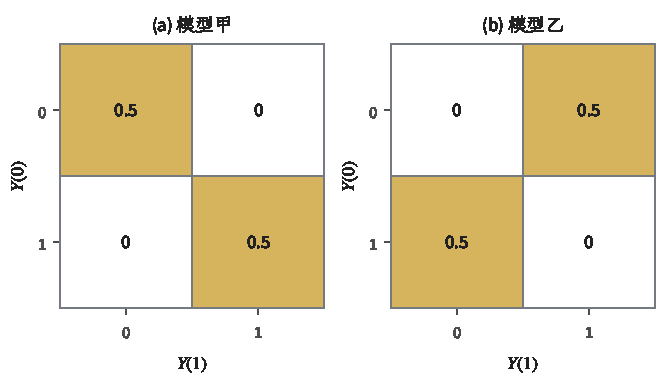
\includegraphics[width=\linewidth]{figures/math-preparation/concept-revision-probability/causal-cross-world-couplings.pdf}
  \caption{相同干预边缘的两种跨世界配对（教学构造的联合概率图）。行对应\(Y(0)\)，列对应\(Y(1)\)，格内数字为联合概率；两图的每个行和、列和均为\(1/2\)。模型甲个体效应恒为零，模型乙个体效应等概率取\(1,-1\)，而两者ATE均为零。这些联合表是相容机制的构造，并非从随机试验中直接观测到的数据。}
  \label{fig:causal-cross-world-couplings}
\end{figure}

两套配对机制连完整随机试验的两组边缘分布也无法区分。若要回答“事实结果为零的这个
单位在另一处理下会怎样”，还需要跨世界联合结构、重复干预、机制限制或相应的部分识别。
这一区别说明，干预分布的点识别不会自动传递给条件个体反事实。

\subsection{输入修改与现实行动}

对一个预测器\(\widehat y=f(\bm{x})\)，把输入字段\(t\)从\(0\)改成\(1\)并重新计算，
只得到
\[
  f(x,t=1)-f(x,t=0).
\]
它描述已训练函数对输入替换的响应。现实行动还可能改变处理的后继变量，并受到资源、
时间和可行域约束。若培训会提高技能，又减少当期工作时间，只修改“是否培训”一列而把
技能和时间固定，通常不是任何可实现世界。

\begin{definition}[因果行动补救]
  \label{def:causal-recourse}
给定事实证据、可实施行动集合\(\mathcal A(x)\)、结构机制、成本\(c(a;x)\)与目标决策集合\(G\)，\term{行动补救}（algorithmic recourse）寻找能使干预后的决策落入\(G\)的可行行动；因果行动补救用同一背景下的干预状态\(\bm V_a\)评价这项成功条件。
\end{definition}
因果补救
需要在结构模型中施加行动，让所有后继变量按机制共同变化，再把新状态送入决策系统。
若事实证据唯一确定了外生背景\(\bm u\)，其优化形式可以写成
\begin{equation}
  \min_{a\in\mathcal{A}(x)}
  c(a;x)
  \quad\text{使得}\quad
  d\bigl(\bm{V}_{a}(\bm{u})\bigr)
  \text{达到目标结果},
  \label{eq:causal-recourse-objective}
\end{equation}
其中\(\mathcal{A}(x)\)是该个体可实施的行动集合，\(c\)是行动成本，
\(\bm{V}_a(\bm{u})\)是同一背景下干预后的状态，\(d\)是最终决策规则。
低输入距离不等于低行动成本，不可改变属性也不应被当作建议。

事实证据通常只给出背景后验
\(P_{\bm U\mid\bm E=\bm e}\)，此时对某个候选\(\bm u\)成功并不保证行动对该个体
可靠。给定可容许失败概率\(\alpha\in[0,1]\)，一种概率型目标是要求
\[
  \mathbb{P}\!\left(
    d(\bm V_a(\bm U))\text{达到目标结果}
    \mid \bm E=\bm e
  \right)
  \geq 1-\alpha.
\]
若要求稳健保证，则可进一步要求后验支持中的每个背景都达到目标。概率约束与最坏情形
约束利用的是同一个背景后验，但后者更保守；二者都比只选一个候选背景检验行动更强。

补救还具有时间和策略边界。多人同时采取建议可能改变价格、名额或审核规则；决策系统
更新后，旧补救未必仍有效；执行成本与成功概率也可能因群体而异。因此，找到一个能翻转
当前模型输出的邻近输入，只证明了当前预测边界的局部性质，不自动证明建议可行、持久或
公平。

\subsection{反事实公平与不可识别性}

反事实公平比较同一个外生背景下，改变受保护属性后预测分布是否保持。设受保护属性为
\(A\)，实际观测为\((X=x,A=a)\)。\begin{definition}[反事实公平]
  \label{def:causal-counterfactual-fairness}
在已指定的SCM与预测规则下，反事实公平要求：对每个允许的替代属性\(a'\)和每个可测预测值集合\(B\)，下列等式对事实证据分布几乎处处的\((x,a)\)成立：
\begin{equation}
  \mathbb{P}\bigl(
    \widehat Y_{A\leftarrow a}\in B
    \mid X=x,A=a
  \bigr)
  =
  \mathbb{P}\bigl(
    \widehat Y_{A\leftarrow a'}\in B
    \mid X=x,A=a
  \bigr).
  \label{eq:causal-counterfactual-fairness}
\end{equation}
\end{definition}
实际观测用于推断背景，随后两个世界共享该背景。只在数据表中替换\(A\)，同时固定所有
由\(A\)产生的后继变量，检验的是不同对象。

个体反事实通常比平均干预效应需要更强结构。第
~\ref{sec:causal-observation-generation}节的两套模型观测分布相同，却对
\(T\leftarrow1\)给出不同后果；即使某些平均效应通过额外设计得到识别，同一个体的
\((Y(0),Y(1))\)联合关系仍可能没有被确定。若多个SCM都与观测和试验结果相容，应在这些
模型上报告反事实或补救结论的范围。一个生成模型能够产出清晰的“另一世界”样本，只说明
它选定了一套机制，不说明该机制已由数据唯一识别。

\section{结构发现与假设检验}
\label{sec:causal-structure-discovery}

前面的效应分析先给定生成结构，再问目标能否识别。本节反过来询问数据能排除哪些结构。
这是推断生成假设的一条独立支线：条件独立只能在Markov性、忠实性与观测制度等条件下
限制候选图，通常不能仅凭观测确定所有箭头方向。它所留下的结构歧义会再进入效应识别。

\subsection{Markov性、忠实性与三点结构}

定义~\ref{def:causal-d-separation}和因果Markov性允许从图推出条件独立。结构发现要
反向利用观测独立性排除候选图，因此还要限制那些由参数巧合产生、却不对应路径阻断的
独立关系。

\begin{definition}[相对于DAG的忠实性]
  \label{def:causal-faithfulness}
  分布\(P\)相对于DAG \(\mathcal G\)满足\term{忠实性}（faithfulness），若对任意两两不交的节点集\(A,B,S\)都有
  \[ \bm V_A\perp\bm V_B\mid\bm V_S
       \quad\Longrightarrow\quad A\perp_{\mathcal G}B\mid S. \]
\end{definition}
它要求分布中出现的条件独立都由图结构解释，而不是由特殊参数抵消、确定性约束或误差相关偶然产生。因果Markov性说明图蕴含
哪些独立性，忠实性允许从观察到的独立性反推图上缺少哪些连接。前者不自动推出后者。

回看图~\ref{fig:causal-local-path-patterns}，面板(a)的共同原因和面板(b)的中介链在
给定中间节点后都会关闭；把中介链的两条箭头同时反向，这一条件独立模式也不变。因此，
忽略节点名称后的三种结构
\(X\to Z\to Y\)、\(X\leftarrow Z\leftarrow Y\)和\(X\leftarrow Z\to Y\)都蕴含
\[
  X\perp Y\mid Z,
\]
并且一般不蕴含\(X\perp Y\)。仅靠这些条件独立关系，无法判断中间变量是传递作用还是
共同原因。相反，面板(c)的碰撞结构通常蕴含\(X\perp Y\)，而给定中间节点后可能相关，
所以可以由不同的独立模式与前三者区分。

\subsection{观测结构与Markov等价类}

\begin{definition}[Markov等价与等价类]
  \label{def:causal-markov-equivalence}
若同一节点集上的两张有向无环图具有完全相同的d-分离关系，就称它们
\term{Markov等价}（Markov equivalent）；与给定图Markov等价的全部有向无环图组成
它的\term{Markov等价类}（Markov equivalence class, MEC）。
\end{definition}
两张图Markov等价，
当且仅当它们具有相同的\term{骨架}（skeleton），即忽略方向后有相同的邻接边，并且
具有相同的\term{无屏蔽碰撞结构}（unshielded collider）：形如
\(X\to Z\leftarrow Y\)，且\(X\)与\(Y\)不相邻\scite{pgm-structure-learning-chickering2002}因而，在因果Markov性与忠实性等
假设下，纯观测条件独立信息通常只能识别一个Markov等价类，而不是唯一有向图。

局部差异已经由图~\ref{fig:causal-local-path-patterns}展示：链和共同原因具有相同骨架，
且都没有无屏蔽碰撞点；碰撞结构则改变了条件化前后的连通模式。对较大图，还要像图
~\ref{fig:causal-d-separation-paths}那样检查全部路径，而不能只比较一个三点片段。
相同骨架且没有新增无屏蔽碰撞点的方向变化，才可能留在同一个等价类中。

必要性要比较全部路径，而不能把一个三点片段当成完整图。在DAG中，非相邻的两点总存在
一个不含端点的d-分离集：选取其中一个节点，使另一点是它的非后代，再以所选节点的父
节点集作分离集。进入所选节点的路径被父节点阻断；从它向外出发而到达非后代的路径必有
一个后代碰撞点，该碰撞点及其后代不可能属于所选节点的父节点集，因而也被阻断。直接
相邻两点之间的单边路径却不能被任何不含端点的集合阻断，所以骨架不同必导致分离关系
不同。

对于无屏蔽三点结构\(X-Z-Y\)，两端不相邻，故存在分离集。若中点不是碰撞点，每个
分离集都必须包含\(Z\)，否则这条长度为二的路径仍开放；若中点是碰撞点，任何分离集
都不能包含\(Z\)，否则该路径被打开。因此，同一骨架上不同的无屏蔽碰撞结构也必定
给出不同分离关系；这个判断允许图中存在其他路径。

充分性需要控制较长路径，这里引用完整的结构判据，不把局部因子重写当作充分性证明
\scite{pgm-structure-learning-chickering2002}下面的覆盖边反转解释已确定的等价类内部
怎样改变方向。一条边\(X\to Y\)若满足
\(\operatorname{pa}(Y)=\operatorname{pa}(X)\cup\{X\}\)，称为
\term{覆盖边}（covered edge）。覆盖边反转定理说明，反转这种边后仍是DAG，且保留
全部d-分离关系\scite{pgm-structure-learning-chickering2002}这一单步变换也可以从相应的两个局部因子理解：
\[
  p(x\mid\operatorname{pa}(X))
  p(y\mid x,\operatorname{pa}(X))
  =
  p(y\mid\operatorname{pa}(X))
  p(x\mid y,\operatorname{pa}(X))
\]
重新表示，不改变它们合起来的条件联合分布。上述等式解释单步的分布重参数化，却还
没有证明两个指定图之间存在整条变换序列。完整的等价类变换定理进一步保证：任意两张
Markov等价DAG均可通过有限次覆盖边反转相互到达，每个中间图都保持无环和等价。
这一变换结论以两图已经Markov等价为前提，说明类内变换的可达性，不能代替上述
结构判据的充分性证明\scite{pgm-structure-learning-chickering2002}

等价类可以用部分有向图表示：在所有等价图中方向一致的边保留箭头，方向仍可变化的边
保持无向。算法输出这种等价类不是“尚未优化好”，而是忠实、无环且无潜在混杂等假设下
观测分布本身留下的总体歧义。增加同一观测分布的样本，只会更准确地判断独立关系，不会
为等价类内部凭空增加方向信息。

\subsection{潜在混杂、选择与有限样本检验}

若所有变量的共同原因都已观测，就称满足因果充分性。潜在共同原因会使两个可观测节点
相关，却无法由其中一方向另一方的箭头正确表示。允许潜在混杂时，结构发现的输出通常要
扩展为带不同端点标记的部分图，用来区分确定的祖先关系、可能方向和无法排除的隐藏共同
原因。测量误差和按碰撞点选择样本也会改变条件独立模式，不能简单解释为新因果边。

总体条件独立在有限样本中还要通过检验或评分近似判断。以
\(H_0:V_i\perp V_j\mid\bm V_S\)为原假设，并假定约束型算法在未拒绝条件独立时
删除候选边：第一类错误把真实独立误判为依赖，可能保留虚假边；第二类错误把实际依赖
误判为独立，可能删除真实边。后续搜索和定向规则还可能传播这些错误，而评分型算法未必
能直接套用这一对应。高维条件集合又使每个分层中的有效样本减少，接近零但非零的依赖
尤其难与独立区分。结构学习的一致性结论需要同时说明真实分布的Markov与忠实条件、
检验或评分随样本增长的性质、候选图范围及搜索是否足以找到目标。算法返回一张确定图，
不代表方向的不确定性已经消失。

\subsection{干预、跨环境信息与方向识别}

干预会切断目标变量原有的进入机制。若在观察数据中\(X\)与\(Y\)相关，而随机设置
\(X\)后\(Y\)的分布随设置值改变，这为\(X\)位于\(Y\)上游提供了观测关联之外的证据。
对不同节点实施干预可以缩小Markov等价类；若干预目标未知、执行不完全或干预同时改变
其他机制，则必须把这些不确定性纳入模型。

跨环境信息也能提供约束。若不同环境只改变少数外生分布，而某个条件机制保持不变，
机制不变性可以帮助比较候选方向。但“关系稳定”单独不是充分条件。隐藏共同原因可能在
所有已观察环境中都稳定，环境变化也可能太弱而没有打破错误方向；选择规则若同步变化，
还可能制造新的稳定关联。应明确哪些机制允许变化、环境标签是否影响结果，以及稳定性
是作为假设、检验对象还是经验线索使用。

结构发现因而需要多类证据协作。条件独立限制观测等价类，受控干预主动打破部分歧义，
机制知识排除不合理方向，敏感性分析检查结论对潜在混杂、弱依赖和选择机制的变化。
这些证据可以互相补充，却不能由一项代理另一项。对于反馈环、随时间变化的机制或处理
定义不稳定的系统，无环静态SCM本身也可能不适用，需要改用动态或循环因果模型并重新
定义干预。

\section{本章小结}
\label{sec:causal-inference-summary}

观测分布描述自然机制运行时变量怎样共同出现，干预分布描述替换某个生成机制后的总体
结果，个体反事实则在实际观测推断出的同一背景下比较另一行动。两套结构机制可以拥有
完全相同的观测分布，却给出不同干预和反事实；这说明预测精度、样本规模和优化能力都
不能代替生成假设。

潜在结果把不同处理下的结果并列表示，一致性连接实际处理与观察结果，无干扰和处理版本
唯一性保证目标定义清楚。随机分配直接建立交换性；观察研究则通常需要条件交换性与支持
重叠。正值性只需覆盖目标总体中目标行动会使用的协变量--行动组合，不要求目标之外处处
重叠。结合这些条件，调整公式和逆概率表示把ATE化成可观测分布的泛函。识别只说明总体
目标能否唯一确定，有限样本估计和数值计算还需各自的误差条件。

当交换性、重叠或机制知识不足时，部分识别保留所有相容答案。有界结果给出不依赖无混杂
的锐界，支持缺口按缺口人群或目标策略未覆盖的概率质量扩大范围，偏差函数把未观测混杂
的强度转成敏感性区间。单调性、效应范围或跨环境机制不变可以收紧集合，但每项收紧都
来自新增假设。一般识别集合未必是区间，上下界只给出它的区间包络；识别集合表达总体
机制歧义，置信区间表达有限样本误差，二者不能混为同一种不确定性。

结构发现同样受识别边界约束。因果Markov性把图结构连接到条件独立，忠实性才允许从独立
关系反推结构；纯观测数据通常只能确定Markov等价类，潜在混杂、选择和测量误差还会扩大
歧义。干预、跨环境变化和机制知识能够补充方向证据，但必须写清各自保持和改变了什么。
因此，因果推断的核心不是为关联加上箭头，而是对每个干预、效应或反事实结论列明目标、
生成假设、可用证据和仍未被决定的范围。此前第~\ref{chap:combinatorics}章已区分
有限候选的计数、可行性、最优性与计算复杂度；接下来的第~\ref{chap:graph-theory}章
会以顶点与边为对象，系统处理路径、分离与图分解。这些图结构可以支持因果图上的计算，
其因果解释仍须由本章的生成与干预假设确定。
第~\ref{chap:decision-theory-and-dynamic-risk}章把单步干预扩展为序贯行动和价值递推；
\BookChapterRef{chap:trust-fairness}{第二卷“基础、理论和可信性”的“公平性”章}与
\BookChapterRef{chap:trust-interpretability}{第二卷“基础、理论和可信性”的“可解释性”章}
则分别回用反事实目标和行动补救，并重新加入规范要求与实际验证条件。
